\chapter{Introduction}\label{chp:resultadosEsparados}

\section{Motivation}

Currently in medicine, surgeries have the objective of causing the least aggression to the patient's organism, which implies a shorter hospitalization time; less incidence of postoperative complications; less pain; and quicker recovery. However, among the many challenges involved in its implementation, the physician's visual ability, which involves the ability to locate and identify sensitive tissues, is essential to reduce damage to the patient during a surgical procedure, leading us to the question: How can we enhance the doctor's vision to increase the quality of these operations?

\begin{figure}[h]
    \centering
    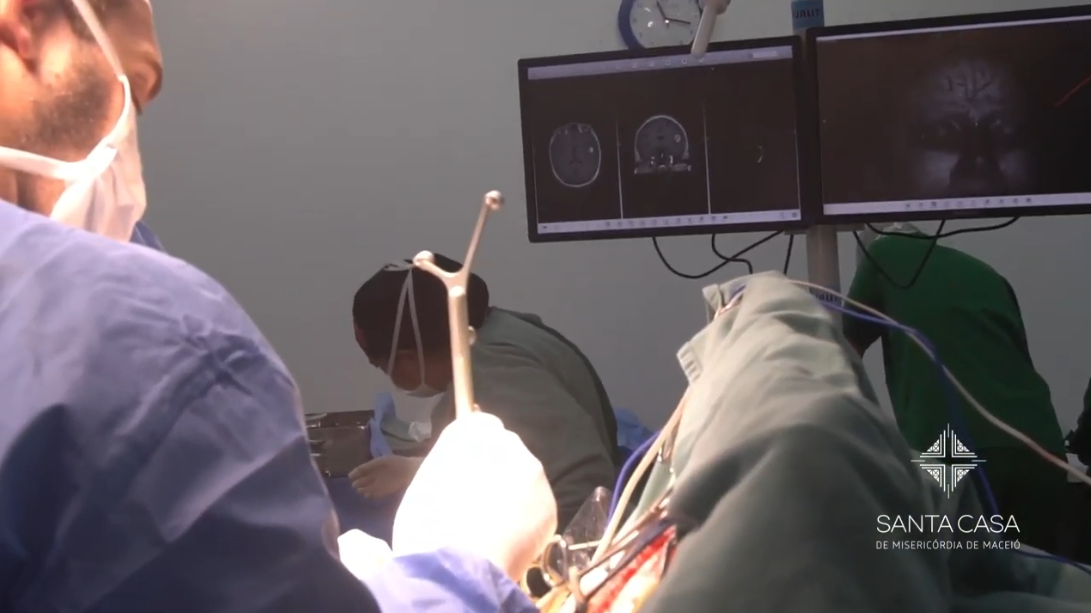
\includegraphics[width=.55\linewidth]{figuras/enunciado.png}
    \caption{Example of using a neuronavigator in surgery. Source: \cite{santacasa}.}
    \label{fig:enunciado}
\end{figure}

To this end, software that informs and assists the doctor in real time during the operation is a great way to increase the chances of success in these surgeries. Currently, these software are very present in the planning and execution of operations, however, neuronavigation systems are an example, whose function is to allow the visualization, in a precise way, of the patient's brain structures. The neurosurgeon has to turn his head to read the monitors and loses focus on the activity being conducted, collaborating for a longer operation time and favoring the exhaustion of the professional, in a way that increases his potential for errors during surgical procedures (Figure \ref{fig:enunciado}).

To do this, augmented reality (AR) technology offers the potential to reduce these limitations, as three-dimensional figures can superimpose the doctor's vision to facilitate visualization and location of the objectives of the operation while keeping their eyes focused on the patient \cite{enhancedvision}. What was done in this project is a research involving computer vision and computer graphics in the field of AR and an application for the glasses of the company Seiko Epson Corporation\textregistered , model Moverio BT-350\texttrademark. Receiving physical and technical support from the Aeronautical Technology Laboratory (Aerotech) team at the University of São Paulo, this study corroborates the group's objective, which is to develop a collaborative neurosurgical multi-application platform.

\section{Objective}

Display information and position three-dimensional models in a region of space with AR, in a way that facilitates the surgeon's access to information during neurosurgery; study and record the response of the equipment used in terms of graphic quality and system response latency. All of this, with the central objective of increasing the proximity of the surgeon to the AR technology as a support during surgical procedures.

% \section{Method}

% Consiste na listagem de possíveis soluções, técnicas ou ferramentas; o estudo e a discussão sobre elas, em seguida, sua implementação. Paralelamente a isso, a busca bibliográfica é constantemente realizada com o objetivo de esclarecer dúvidas sobre os meios imaginados e discutidos com o orientador e coorientador. Essa busca enfatiza os resultados encontrados pelos artigos, o objetivo disto é caracterizar os prós e contras das diversas opções encontradas. Essa pesquisa de artigos trás uma evolução do discernimento dos assuntos do estado da arte, refletindo em uma noção de funcionamento dos métodos científicos que constrói um novo pesquisador no desenvolvimento dessa iniciação científica.

\section{Brief history of the project}

\begin{figure}[H]
\centering
    \begin{subfigure}{0.45\textwidth}
        \centering
        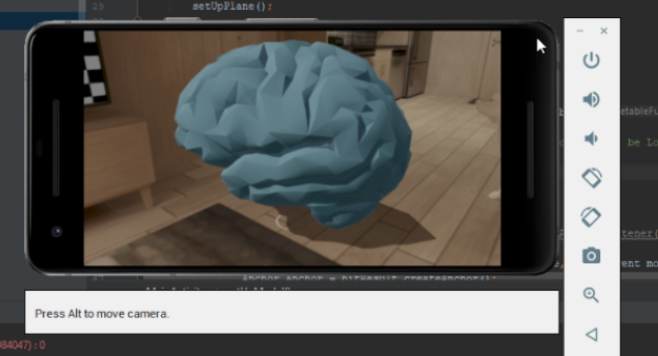
\includegraphics[width=.95\textwidth]{figuras/sceneform.png}
        \caption{First AR app for Android}
        \label{fig:sceneform}
    \end{subfigure}
    \begin{subfigure}{0.45\textwidth}
        \centering
        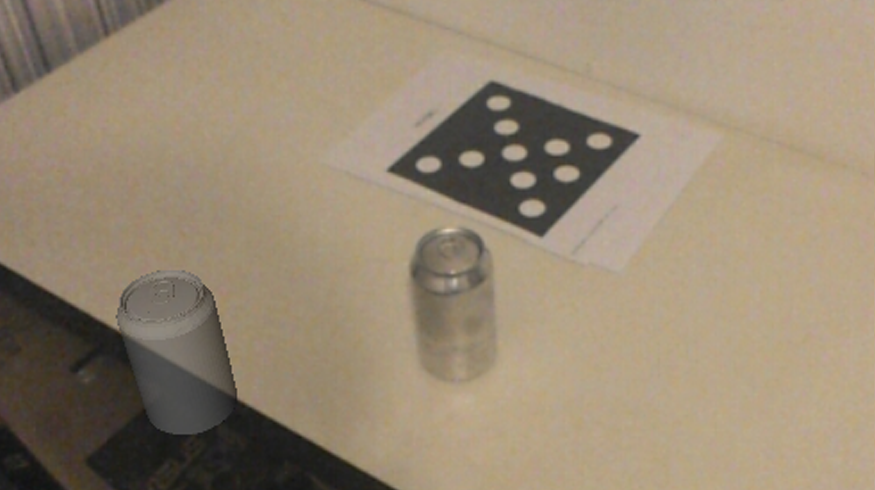
\includegraphics[width=.95\linewidth]{figuras/Latinha-errada.png}
        \caption{Moverio calibration attempt}
        \label{fig:latinha}
    \end{subfigure}
    \begin{subfigure}{0.45\textwidth}
        \centering
        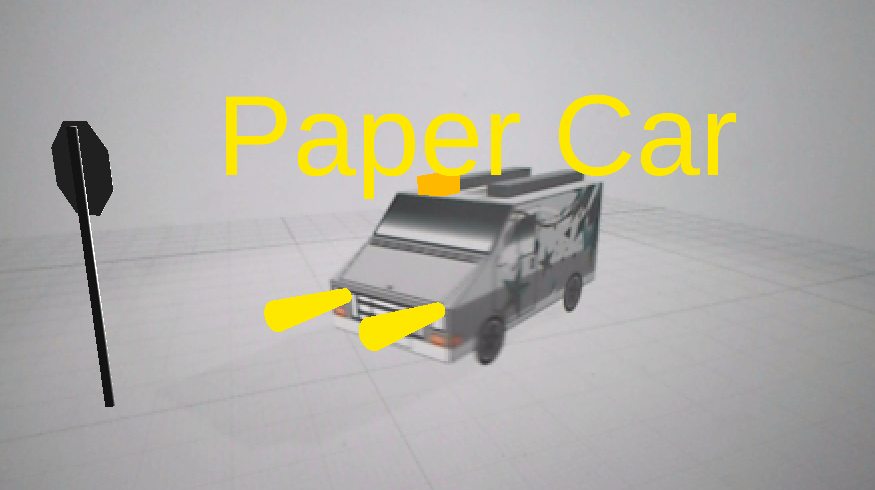
\includegraphics[width=.95\textwidth]{figuras/PaperCarAR.png}
        \caption{Application provided by EPSON}
        \label{fig:papercar}
    \end{subfigure}
    \begin{subfigure}{0.45\textwidth}
        \centering
        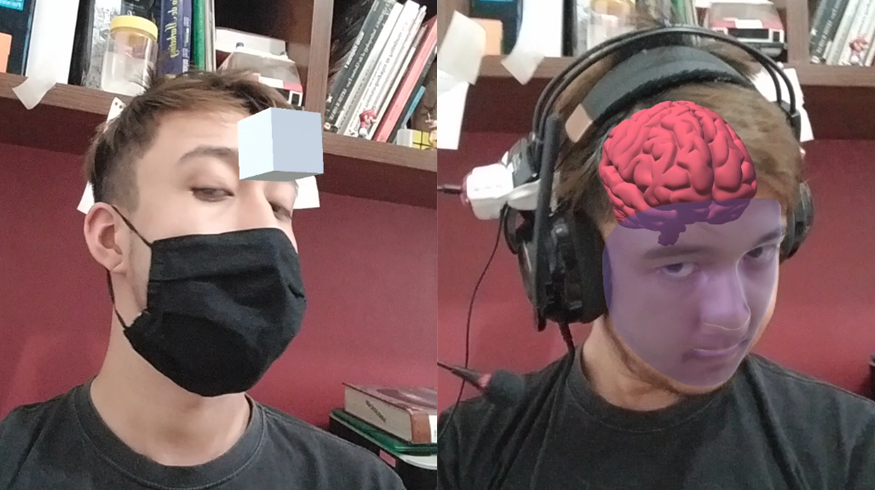
\includegraphics[width=.95\linewidth]{figuras/VCranium.png}
        \caption{First version of VCranium}
        \label{fig:vcranium_alpha}
    \end{subfigure}
    \caption{History of research since 2020.}
    \label{fig:historico}
\end{figure}

Since the beginning of work on the project in 2020, different types of contact have been experienced with the development of software for the Android operating system (Figure \ref{fig:sceneform}); tests of the Moverio BT-350 augmented reality glasses documentation tools (Figures \ref{fig:latinha} and \ref{fig:papercar}); and the creation of applications that illustrate the purpose of VCranium \footnote[1]{Fantasy name assigned to the project of positioning system and display of augmented reality for surgical application} (Figure \ref{fig:vcranium_alpha}).